\section{Modelo de Pré-Viabilidade Financeira de PPP's}
\label{sec:modelo-de-pre-viabilidade-financeira-de-ppps}

O modelo desenvolvido nesta etapa tem como objetivo fazer uma análise preliminar da viabilidade financeira de um projeto de PPP. A análise da planilha que representa o modelo baseia-se na metodologia “Value for Money”, fazendo primeiramente um levantamento da taxa WACC (Weighted Average Cost of Capital)\footnote{Há de se destacar que uma abordagem largamente utilizada no Brasil é o uso de um modelo de referência para apreçamento de ativos e fluxo de caixa, notoriamente o modelo CAPM (Capital Asset Pricing Model) é usualmente utilizado para avaliar as implicações de transferências de risco no contexto de PPPs. Para avaliar robustez dos resultados, outros modelos concorrentes (como modelos de arbitragem e teoria de portfólio de Merton ) e modelos estocásticos (simulação de Monte Carlo) também são empregados para apreçamento de ativos para efeitos comparativos e seleção do melhor método.}  através de dados disponíveis para consulta pública e coletados através de um script em linguagem de programação R. Obtida tal taxa, a planilha recebe como entrada um conjunto reduzido de dados do projeto e, com base neles, avalia se há vantagem financeira em realizar o projeto pela modalidade PPP ou se é mais interessante a execução do mesmo através de um processo licitatório comum.

\subsection{Revisão de Literatura}
\label{subsec:revisao-da-literatura}

O desenvolvimento desta ferramenta baseia-se fortemente na análise conhecida como “Value for Money” (VfM) aqui definida, simplificadamente, como uma medida do tamanho da redução de custo alcançada ao entregar um projeto através da modalidade PPP em relação à abordagem tradicional realizada pelo setor público (FAROOQI e SIEMIATYCKI, 2012). Em um estudo conduzido pela OCDE, conclui-se que 19 de 20 países pesquisados utilizam algum tipo de análise VfM nos processos de avaliação de opção de PPP (BURGER e HAWKESWORTH, 2011, apud SOARES JÚNIOR, 2019, p. 26). A Figura 1 resume o processo de análise VfM, no qual dois cenários são estabelecidos: PPP (Parceria Público-Privada) e OSP (Opção do Setor Público), também conhecido como PSC (Public Sector Comparator).

\begin{figure}[ht!]
    \centering
    \caption{Quadro unificado para opções de contratação pública.}
    \label{fig:estrutura-de-impostos}
    \IBGEtab{}{
	     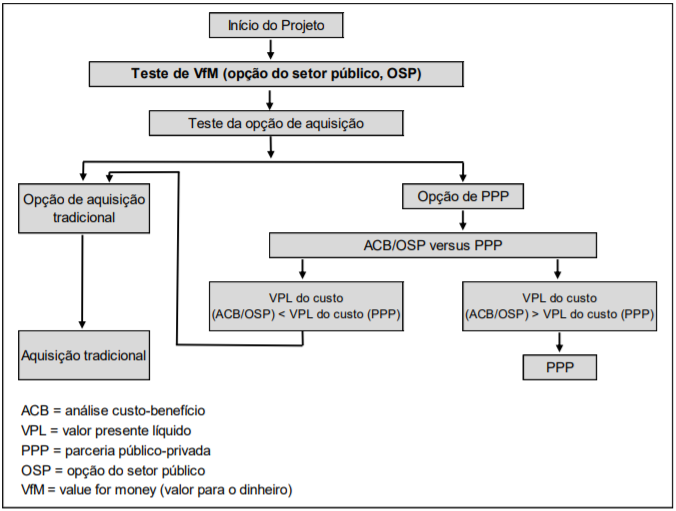
\includegraphics[width=0.8\textwidth]{figuras/figura1.png}
	}{
	    \Fonte{BURGER e HAWKESWORTH, 2011, p. 48, apud SOARES JÚNIOR, 2019, p. 26.}
	}
\end{figure}

Para ambos os cenários, é calculado o VPL (Valor Presente Líquido) do projeto, sendo posteriormente comparados. Caso o VPL do cenário OSP seja maior do que o VPL do cenário PPP, recomenda-se a opção de aquisição tradicional pelo setor público (geralmente, no caso brasileiro, o procedimento licitatório comum regido pela Lei 8.666/93). Caso contrário, a análise VfM indica, portanto, a entrega do projeto pela modalidade PPP. O cálculo do Valor Presente Líquido, por sua vez, é efetuado utilizando a taxa WACC (Weighted Average Cost of Capital) como fator de desconto:

\begin{citacao}
De acordo com os custos de cada fonte de financiamento (própria e não própria) da empresa, é importante que se determine seu custo total de capital principalmente para melhor orientar suas decisões financeiras. O custo total de capital, conforme foi comentado, representa a taxa de atratividade da empresa, que indica a remuneração mínima que deve ser exigida na alocação de capital, de forma a maximizar seu valor de mercado. O cálculo desse custo é processado pelo critério da média ponderada. (ASSAF NETO, 2014, p. 481).
\end{citacao}

Segundo Assaf Neto (2014), podemos obter o custo médio ponderado do capital (WACC) através da seguinte fórmula:
\begin{equation}
    ACC=\sum_{j=1}^{N}W_j\times K_j
\end{equation}
onde: $WACC$ é o custo médio ponderado do capital; $W_j$ = participação relativa de cada fonte de capital no financiamento total; $K_j$ = custo específico de cada fonte de financiamento (própria e de terceiros).

\subsection{Material Utilizado}

A planilha está sendo desenvolvida, em sua grande parte, no software Microsoft Excel evitando, no entanto, a utilização de extensões e ferramentas que possam torná-la incompatível com softwares livres, tais como o Libre Office. Diversos cuidados estão sendo tomados para garantir a simplicidade do uso por parte do usuário, bem como a transparência nos métodos utilizados. A planilha, no estágio atual de desenvolvimento, recebe um conjunto simplificado de dados referentes ao projeto, tais como duração (em anos), remuneração, previsão de demanda, dentre outros. Ao montar dois cenários (PPP e PSC), a planilha calcula o VPL (Valor Presente Líquido) das duas situações considerando a taxa de desconto dada pelo WACC (Custo Médio Ponderado do Capital). 

O cálculo desta taxa, por sua vez, é realizado de maneira independente por um script desenvolvido na linguagem de programação R (Anexo). O objetivo do script é automatizar a rotina de obtenção e processamento de dados de diversas fontes. Como bases de dados para o cálculo da taxa WACC são utilizadas as planilhas de custos de capital por setor da indústria (DAMODARAN, 2020a), de betas alavancados e desalavancados por indústria (DAMODARAN, 2020b) e de dados do mercado acionário dos EUA de 1871 até o presente \cite{o2020using}. Além destas, duas séries temporais também são utilizadas: o risco-brasil medido pelo índice EMBI+ (IPEADATA, 2020a) e o índice de preços ao consumidor dos EUA dessazonalizado (IPEADATA, 2020b). Ao terminar o cálculo, o script retorna um arquivo .csv com os resultados obtidos o qual é, por sua vez, importado pela planilha.

Para o cálculo da taxa WACC do projeto, supõe-se que este tenha uma estrutura de capital tal como Damodaran (2020a) e que o beta desalavancado do setor seja o dado por Damodaran (2020b). O beta é, então, realavancado:

$$\beta_l=\beta_u\left[1+(1-\tau)\frac{w_d}{W_e}\right]$$
Onde: $\beta_l$ = beta realavancado do setor; $\beta_u$ = beta desalavancado do setor; $\tau$ = impostos incidentes, tais como Imposto de Renda (IR) e Contribuição Social sobre o Lucro Líquido (CSLL); $W_d$ = percentual de capital de terceiros; $W_e$ = percentual de capital próprio.

Utilizam-se as seguintes fórmulas para a obtenção do custo específico do capital próprio e do capital de terceiros:
\begin{align}
    K_e&=R_f+\beta_l(R_m-R_f)+R_{BR} \\
    K_d&=R_f+C_d+R_{BR}
\end{align}
onde: $K_e$ = custo de capital próprio (nominal); $R_f$ = taxa livre de risco (taxa média anual dos retornos dos títulos americanos com prazo de 10 anos); $\beta_l$ = beta realavancado do setor; $R_m$ = retorno de mercado (taxa média anual dos retornos de uma carteira composta pelas ações listadas no índice S&P 500); $Prêmio$ = prêmio de mercado, dado pela diferença entre o retorno de mercado e a taxa livre de risco; $R_BR$ = risco sistêmico (mediana do risco-brasil diário mensurado pelo índice EMBI+); $K_d$ = custo de capital de terceiros (nominal); $C_d$ = custo de capital de terceiros de empresas do setor nos EUA.

Os valores são trazidos para termos reais, de acordo com a inflação mensurada pelo índice de preços ao consumidor dos EUA (IPEADATA, 2020b):
\begin{align}
    \overline{K}_e&=\frac{1+K_e}{1+\pi_{EUA}} \\
    \overline{K}_d&=\frac{1+K_d}{1+\pi_{EUA}}
\end{align}
onde: $\overline{K}_e$ = custo de capital próprio (real);  $K_e$ = custo de capital próprio (nominal); $\overline{K}_d$ = custo de capital de terceiros (real); $K_d$ = custo de capital terceiros (nominal); $\pi_{EUA}$ = inflação dos EUA (mediana da variação percentual anual do índice de preços ao consumidor dos EUA).

Por fim, obtém-se a taxa WACC:
\begin{align}
    WACC=W_e\overline{K}_e+(1-\tau)W_d\overline{K}_d
\end{align}
onde $WACC$ = custo médio ponderado do capital; $W_e$ = percentual de capital próprio; $\overline{K}_e$ = custo de capital próprio (real); $W_d$ = percentual de capital de terceiros; $\overline{K}_d$ = custo de capital de terceiros (real); $\tau$ = impostos incidentes.

Como resultado, a planilha fornece o fluxo de caixa descontado dos dois cenários, considerando as suposições dadas na entrada e a taxa WACC obtida via script. A situação que fornecer o melhor VPL é, portanto, indicada como a melhor. A aplicação do modelo é em comparar os resultados apresentados pelos proponentes para a CGPPP com uma metodologia padrão, havendo a flexibilidade em analisar sensibilidade há mudança de cenários de risco e a desconhecimento de custos aventados pelo proponente. Saliente-se que estes pontos são relatados na literatura quanto aos FCS, o que deixa a SEPLAG mais confortável em avaliar riscos prévios com base na experiência internacional relatado no Produto 1.






